\section{Prerequisitos}

\subsection{¿Qué es un contenedor?}

Un contenedor es una unidad estandarizada de software que empaqueta código y todas sus dependencias para que una aplicación se ejecute de forma rápida, confiable y consistente en diferentes entornos. Es una forma ligera, portátil y aislada de ejecutar procesos o aplicaciones.

\subsubsection{Componentes clave de un contenedor}
\begin{itemize}
    \item \textbf{Aplicación principal}: El binario o script que se quiere ejecutar.
    \item \textbf{Dependencias}: Librerías, módulos, herramientas del sistema necesarias.
    \item \textbf{Sistema de archivos aislado}: Un entorno controlado, consistente y separado del sistema operativo anfitrión.
    \item \textbf{Red y procesos aislados}: Gracias a tecnologías como \textit{cgroups} y \textit{namespaces} del kernel de Linux.
    \item \textbf{Capacidad de ser portado}: Se comporta igual en desarrollo, pruebas o producción.
\end{itemize}

\subsubsection{Creación y gestión de contenedores}
Para crear y gestionar contenedores, se utilizan herramientas como:

\paragraph{Docker:}
\begin{itemize}
    \item Permite construir imágenes (plantillas de contenedor) y lanzar contenedores a partir de ellas.
    \item Una \textit{imagen Docker} es como una instantánea de un sistema preconfigurado.
    \item Un \textit{contenedor Docker} es una instancia en ejecución de esa imagen.
\end{itemize}

\paragraph{Podman:}
\begin{itemize}
    \item Alternativa moderna a Docker, compatible con sus comandos, pero no necesita un \textit{daemon} (demonio) en segundo plano.
    \item Cada contenedor se ejecuta como un proceso del usuario, lo cual es más seguro en entornos multiusuario.
    \item Soporta \textit{rootless containers} (contenedores sin privilegios de administrador).
\end{itemize}

\subsubsection{¿Qué es Docker Compose?}
Docker Compose es una herramienta que permite definir y ejecutar múltiples contenedores Docker mediante un archivo YAML (\texttt{docker-compose.yml}). Es ideal para sistemas distribuidos o aplicaciones que requieren múltiples servicios, como una aplicación web con base de datos y servidor de caché.

\textbf{Ejemplo básico:}
\begin{lstlisting}[style=customstyle]
version: '3'
services:
  web:
    image: nginx
    ports:
      - "80:80"
  db:
    image: postgres
    environment:
      POSTGRES_PASSWORD: example
\end{lstlisting}

Este archivo lanza dos contenedores: uno con Nginx y otro con PostgreSQL, conectados en una red compartida automáticamente gestionada por Docker Compose.

\subsubsection{Diferencias entre Docker, Docker Compose y Podman}
\begin{table}[h!]
\centering
\begin{tabular}{|p{3cm}|p{3cm}|p{3cm}|p{3cm}|}
\hline
\textbf{Característica} & \textbf{Docker} & \textbf{Docker Compose} & \textbf{Podman} \\ \hline
Motor de contenedores & Sí & Usa Docker & Sí \\ \hline
Ejecuta múltiples contenedores & No directamente & Sí, orquestación básica & Sí, con \texttt{podman-compose} \\ \hline
Requiere daemon & Sí & Sí (usa Docker) & No \\ \hline
Rootless & Limitado & No & Sí, por diseño \\ \hline
Compatible con Dockerfiles & Sí & Sí & Sí \\ \hline
\end{tabular}
\end{table}

\subsubsection{Resumen conceptual}
Un contenedor no es una máquina virtual. No tiene su propio kernel ni simula hardware. Comparte el kernel del sistema anfitrión, lo que lo hace mucho más ligero y rápido, ideal para microservicios, DevOps y CI/CD.

Docker Compose y Podman son formas de gestionar contenedores: la primera, muy útil para múltiples servicios coordinados; la segunda, más flexible, más segura y sin necesidad de \textit{daemon}, orientada a usuarios avanzados y producción segura.

\subsection{Ejemplos}
\begin{itemize}
    \item Crear un contenedor con Docker: \texttt{docker run -d -p 80:80 nginx}
    \item Crear un contenedor con Podman: \texttt{podman run -d -p 80:80 nginx}
    \item Usar Docker Compose para lanzar múltiples servicios: \texttt{docker-compose up}
\end{itemize}

\subsubsection{Comparativa con una MV}

\subsubsection{Contenedor vs Máquina Virtual}

Tanto los contenedores como las máquinas virtuales aíslan aplicaciones del sistema anfitrión, pero lo hacen de formas muy diferentes.

\paragraph{Similitudes:}
Ambos permiten ejecutar aplicaciones en entornos separados, evitando que interfieran con el sistema principal.

\paragraph{Diferencias principales:}
\begin{table}[h!]
\centering
\begin{tabular}{|p{5cm}|p{5cm}|p{5cm}|}
\hline
\textbf{Característica}         & \textbf{Máquina Virtual}                     & \textbf{Contenedor}                     \\ \hline
Sistema Operativo               & Incluye su propio sistema operativo          & Comparte el kernel del anfitrión         \\ \hline
Peso                            & Pesado: varios GBs                           & Ligero: pocos MBs                        \\ \hline
Arranque                        & Lento (minutos)                              & Rápido (segundos o menos)                \\ \hline
Consumo de recursos             & Alto: CPU, RAM, disco                        & Bajo y eficiente                         \\ \hline
Virtualización                  & A nivel de hardware (hipervisor)             & A nivel de sistema operativo (namespaces) \\ \hline
Portabilidad                    & Limitada (por sistema operativo)             & Muy alta (misma imagen funciona en múltiples sistemas) \\ \hline
Ideal para                      & Emular sistemas completos, testing de OS     & Desarrollar y desplegar aplicaciones     \\ \hline
\end{tabular}
\end{table}

\paragraph{Analogía:}
Imagina un edificio:
\begin{itemize}
    \item Una máquina virtual es como un departamento completo: tiene su propio baño, cocina y sistema eléctrico. Es independiente, pero consume más recursos.
    \item Un contenedor es como una habitación en un mismo piso: tiene sus propios muebles y decoración (aplicación y dependencias), pero comparte el sistema de agua, luz y estructura (el kernel del sistema operativo).
\end{itemize}

\paragraph{Conclusión:}
Un contenedor es similar a una máquina virtual, pero más ligero y rápido porque no incluye un sistema operativo completo. Esto lo hace ideal para desarrollo, pruebas, despliegue continuo y microservicios.

\subsection{Instalación de Docker y Docker Compose}

A continuación, se presenta una guía detallada para instalar Docker y Docker Compose en Ubuntu 24.04, sin utilizar Docker Desktop, lo que resulta en una instalación más ligera y estable.

\subsubsection{1. Preparar el sistema}

Abra una terminal y actualice el sistema:

\begin{lstlisting}[style=customstyle]
sudo apt update && sudo apt upgrade -y
\end{lstlisting}

Instale las herramientas necesarias:

\begin{lstlisting}[style=customstyle]
sudo apt install ca-certificates curl gnupg lsb-release -y
\end{lstlisting}

\subsubsection{2. Agregar la clave GPG oficial de Docker}

Cree el directorio para almacenar la clave:

\begin{lstlisting}[style=customstyle]
sudo mkdir -p /etc/apt/keyrings
\end{lstlisting}

Descargue y almacene la clave GPG oficial de Docker:

\begin{lstlisting}[style=customstyle]
curl -fsSL https://download.docker.com/linux/ubuntu/gpg | sudo gpg --dearmor -o /etc/apt/keyrings/docker.gpg
\end{lstlisting}

\subsubsection{3. Agregar el repositorio oficial de Docker}

Agregue el repositorio de Docker a la lista de fuentes de APT:

\begin{lstlisting}[style=customstyle]
echo \
    "deb [arch=$(dpkg --print-architecture) signed-by=/etc/apt/keyrings/docker.gpg] \

    https://download.docker.com/linux/ubuntu \
    $(lsb_release -cs) stable" | \
    sudo tee /etc/apt/sources.list.d/docker.list > /dev/null
\end{lstlisting}

\subsubsection{4. Instalar Docker Engine y Docker Compose}

\textbf{Nota: Es para nuestra máquina (ubuntu).}

Actualice los paquetes e instale Docker y Docker Compose:

\begin{lstlisting}[style=customstyle]
sudo apt update
sudo apt install docker-ce docker-ce-cli containerd.io docker-buildx-plugin docker-compose-plugin -y
\end{lstlisting}

\subsubsection{5. Verificar que Docker está funcionando}

Ejecute los siguientes comandos para verificar la instalación:

\begin{lstlisting}[style=customstyle]
sudo docker version
sudo docker info
\end{lstlisting}

Si se muestra información sobre Docker, la instalación fue exitosa.

\subsubsection{6. (Opcional) Ejecutar Docker sin \texttt{sudo}}

Para permitir que Docker se ejecute sin necesidad de usar \texttt{sudo}, ejecute:

\begin{lstlisting}[style=customstyle]
sudo usermod -aG docker $USER
\end{lstlisting}


Acto seguido, cierre la sesión y vuelva a iniciarla para que los cambios surtan efecto.
\begin{lstlisting}[style=customstyle]
sudo systemctl restart docker
\end{lstlisting}

\textbf{Nota:} Cierre la sesión y vuelva a iniciarla (o reinicie el sistema) para que los cambios surtan efecto.

\subsection{Guía rápida de prueba}

\subsubsection{1. Probar Docker}

Ejecute el siguiente comando para probar Docker:

\begin{lstlisting}[style=customstyle]
docker run hello-world
\end{lstlisting}

Debería aparecer un mensaje indicando que Docker está instalado correctamente.

\subsubsection{2. Probar Docker Compose}

Cree una carpeta de prueba y acceda a ella:

\begin{lstlisting}[style=customstyle]
mkdir docker-prueba && cd docker-prueba
\end{lstlisting}

Cree un archivo \texttt{docker-compose.yml}:

\begin{lstlisting}[style=customstyle]
nano docker-compose.yml
\end{lstlisting}

Pegue el siguiente contenido en el archivo:

\begin{lstlisting}[style=customstyle]
version: "3.8"
services:
    web:
        image: nginx
        ports:
            - "8080:80"
\end{lstlisting}

Guarde y cierre el archivo. Luego, ejecute el servicio:

\begin{lstlisting}[style=customstyle]
docker compose up -d
\end{lstlisting}

Abra un navegador y acceda a \texttt{http://localhost:8080}. Debería visualizar la página de bienvenida de NGINX.

Para detener el servicio, ejecute:

\begin{lstlisting}[style=customstyle]
docker compose down
\end{lstlisting}

Con estos pasos, Docker y Docker Compose estarán instalados y funcionando correctamente.

\subsection{Instalación de Docker Engine en Rocky Linux 9 (o CentOS Stream 9)}

Esta guía es ideal para máquinas virtuales (MV) sin entorno gráfico.

\subsubsection{Paso 1: Preparar el sistema}

Actualice el sistema con los siguientes comandos:

\begin{lstlisting}[style=customstyle]
sudo dnf update -y
sudo dnf upgrade -y
\end{lstlisting}

Instale los paquetes necesarios:

\begin{lstlisting}[style=customstyle]
sudo dnf install -y dnf-utils device-mapper-persistent-data lvm2
\end{lstlisting}

\subsubsection{Paso 2: Agregar el repositorio oficial de Docker}

Agregue el repositorio oficial de Docker con el siguiente comando:

\begin{lstlisting}[style=customstyle]
sudo dnf config-manager --add-repo https://download.docker.com/linux/centos/docker-ce.repo
\end{lstlisting}

\textbf{Nota:} Docker no ofrece repositorios específicos para Rocky Linux, pero el de CentOS funciona perfectamente.

\subsubsection{Paso 3: Instalar Docker Engine}

Instale Docker Engine y sus componentes:

\begin{lstlisting}[style=customstyle]
sudo dnf install -y docker-ce docker-ce-cli containerd.io docker-buildx-plugin docker-compose-plugin
\end{lstlisting}

\subsubsection{Paso 4: Habilitar y arrancar el servicio Docker}

Habilite y arranque el servicio Docker con los siguientes comandos:

\begin{lstlisting}[style=customstyle]
sudo systemctl enable docker
sudo systemctl start docker
\end{lstlisting}

\subsubsection{Paso 5: Verificar la instalación}

Verifique que Docker se instaló correctamente ejecutando:

\begin{lstlisting}[style=customstyle]
docker --version
\end{lstlisting}

Debería mostrar una salida similar a:

\texttt{Docker version 24.x.x, build xxxxxxx}

\subsubsection{Paso 6: Permitir el uso de Docker a usuarios no root}

Para permitir que Docker se ejecute sin necesidad de usar \texttt{sudo}, siga estos pasos:

\begin{enumerate}
    \item Cree el grupo \texttt{docker} (si no existe):
    \begin{lstlisting}[style=customstyle]
sudo groupadd docker
    \end{lstlisting}
    \item Añada su usuario al grupo:
    \begin{lstlisting}[style=customstyle]
sudo usermod -aG docker $USER
    \end{lstlisting}
    \item Cierre la sesión y vuelva a iniciarla para aplicar los cambios.
\end{enumerate}

Pruebe que Docker se ejecuta sin \texttt{sudo} ejecutando:

\begin{lstlisting}[style=customstyle]
docker run hello-world
\end{lstlisting}


\section{Microservicios}

La arquitectura de microservicios es un enfoque de desarrollo de software en el que una aplicación se descompone en un conjunto de pequeños servicios independientes que se comunican entre sí mediante APIs o sistemas de mensajería como RabbitMQ, Kafka o Qpid. Cada microservicio está diseñado para encargarse de una funcionalidad específica del sistema y puede desarrollarse, desplegarse y escalarse de manera autónoma.

Este modelo ha ganado popularidad con el auge de los contenedores, ya que facilita el despliegue y la gestión de estos servicios de forma independiente. Entre sus principales ventajas destacan:

\begin{itemize}
    \item \textbf{Flexibilidad:} Cada servicio puede utilizar su propio stack tecnológico, adaptándose mejor a sus necesidades específicas.
    \item \textbf{Escalabilidad:} Permite escalar verticalmente (mejorando los recursos de un servicio) u horizontalmente (añadiendo instancias del servicio según la demanda).
\end{itemize}

Para más información sobre esta arquitectura, se recomienda consultar el artículo de Martin Fowler: \href{https://martinfowler.com/articles/microservices.html}{Microservices}.

\section{Ejercicio Evaluable. Ejecutar “Hello World”}

Instale Docker en su ordenador anfitrión o en una MV y ejecute el contenedor
``Hello World'' disponible en: \href{https://hub.docker.com/_/hello-world}.

Para ello debemos de ejecutar los siguientes comandos:

\begin{enumerate}[label=\textbf{\arabic*:}]
    \item \micode{sudo docker version}: para ver si docker está instalado correctamente.
    \item \micode{sudo docker run hello-world}: para ejecutar el contenedor. (Ver figura \ref{fig:hello-world})
\end{enumerate}

\begin{figure}[H]
    \centering
    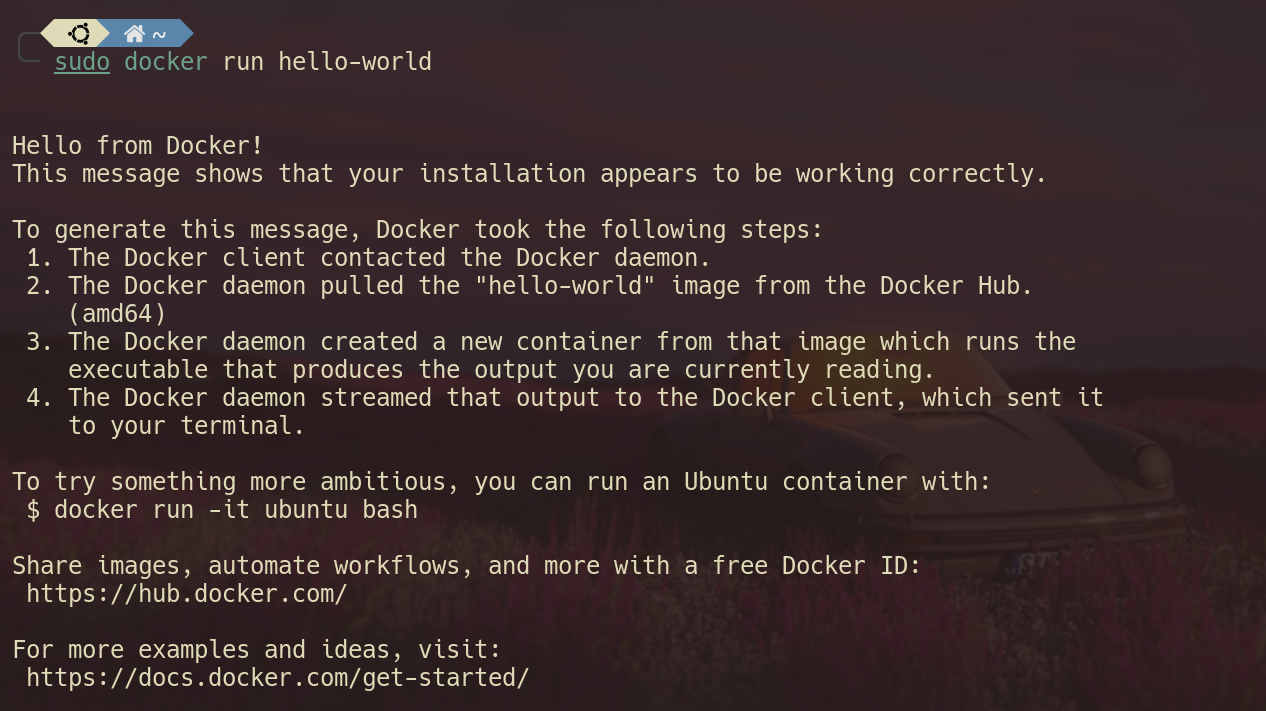
\includegraphics[width=0.8\textwidth]{images/Bloque2/hello-world.png}
    \caption{Contenedor Hello World}
    \label{fig:hello-world}
\end{figure}

\section{BenchMarks}






